\section{Survey Design and Observations}
\label{sec:survey}

\subsection{Telescope and calibrated measurements}
\label{sec:facility}

\SHARP\ uses the 60/90~cm Schmidt telescope at Xinglong Observatory,
with a 0.60~m effective aperture and an $f/3$ optical system. The camera
was developed at the National Astronomical Observatories, Chinese
Academy of Sciences. Its CCD contains $9,216\times9,232$ pixels of
$10~\mu$m, read through 16 simultaneous output channels. A typical
scale of $1.15\asec$~pixel$^{-1}$ gives a nominal
$2.94^\circ\times2.95^\circ$ field of view. The observatory has Minor
Planet Center (MPC) code 327. Table~\ref{tab:design} lists the instrument
and observing parameters used for the standard survey.

Image reduction includes bias and flat-field correction, astrometric
calibration, source extraction, and photometric calibration
\citep[in preparation]{Li2026InPrep}. Astrometry is tied to Gaia EDR3
\citep{GaiaEDR32021,Lindegren2021EDR3}. Reference ICRS positions at
J2016.0 are advanced to the Julian year of the UTC exposure start using
the catalog proper motions and Astropy \citep{Astropy2022}, with
$\mu_\alpha\cos\delta$ used for the right-ascension component. The
propagation uses position and proper motion; stars with unavailable
propagated coordinates retain their catalog positions. SCAMP
\citep{Bertin2006SCAMP} fits a TPV astrometric solution to the propagated
reference positions. Source positions are then evaluated from the
image world coordinate system (WCS), and fixed circular-aperture
photometry is measured with SExtractor \citep{BertinArnouts1996}.
Figure~\ref{fig:exposure} illustrates a standard survey exposure.

The observations considered here use white light, denoted $W$ in the
observing records. We write the calibrated eight-pixel-diameter aperture
magnitude as \gaper; its aperture radius is approximately $4.60\asec$.
The photometric reference scale uses a fixed cubic transformation of
Gaia EDR3 $G$ and $G_{\rm BP}-G_{\rm RP}$
\citep{Riello2021EDR3,Li2026InPrep},
\begin{equation}
W_{\rm ref}=G+\Delta_W+P_W(C-C_0),\qquad
C=G_{\rm BP}-G_{\rm RP},
\label{eq:color}
\end{equation}
where $P_W$ is the adopted color polynomial and $\Delta_W$ and $C_0$
are fixed calibration constants. The white-light reference-star
match uses the original Gaia catalog coordinates. Thus the
astrometric solution and the photometric reference-star selection
use different coordinate epochs.

The zero point $ZP$ is the clipped median difference between the
reference and instrumental magnitudes measured in an 18-pixel-diameter
aperture. For an eight-pixel-diameter source flux $f_8$ in ADU, the
reported magnitude is
\begin{equation}
\gaper=ZP-2.5\log_{10}f_8+C_8,
\label{eq:apercal}
\end{equation}
where $C_8$ is the median difference between the instrumental
18-pixel and eight-pixel aperture magnitudes of the reference stars.
The corresponding flux correction also scales the flux uncertainty.
Throughout this paper, \gaper\ denotes this white-light scale.
Comparisons with asteroid $V$ magnitudes or standard photometric
bands depend on the source color and system response.

\begin{figure}[tbp]
\centering
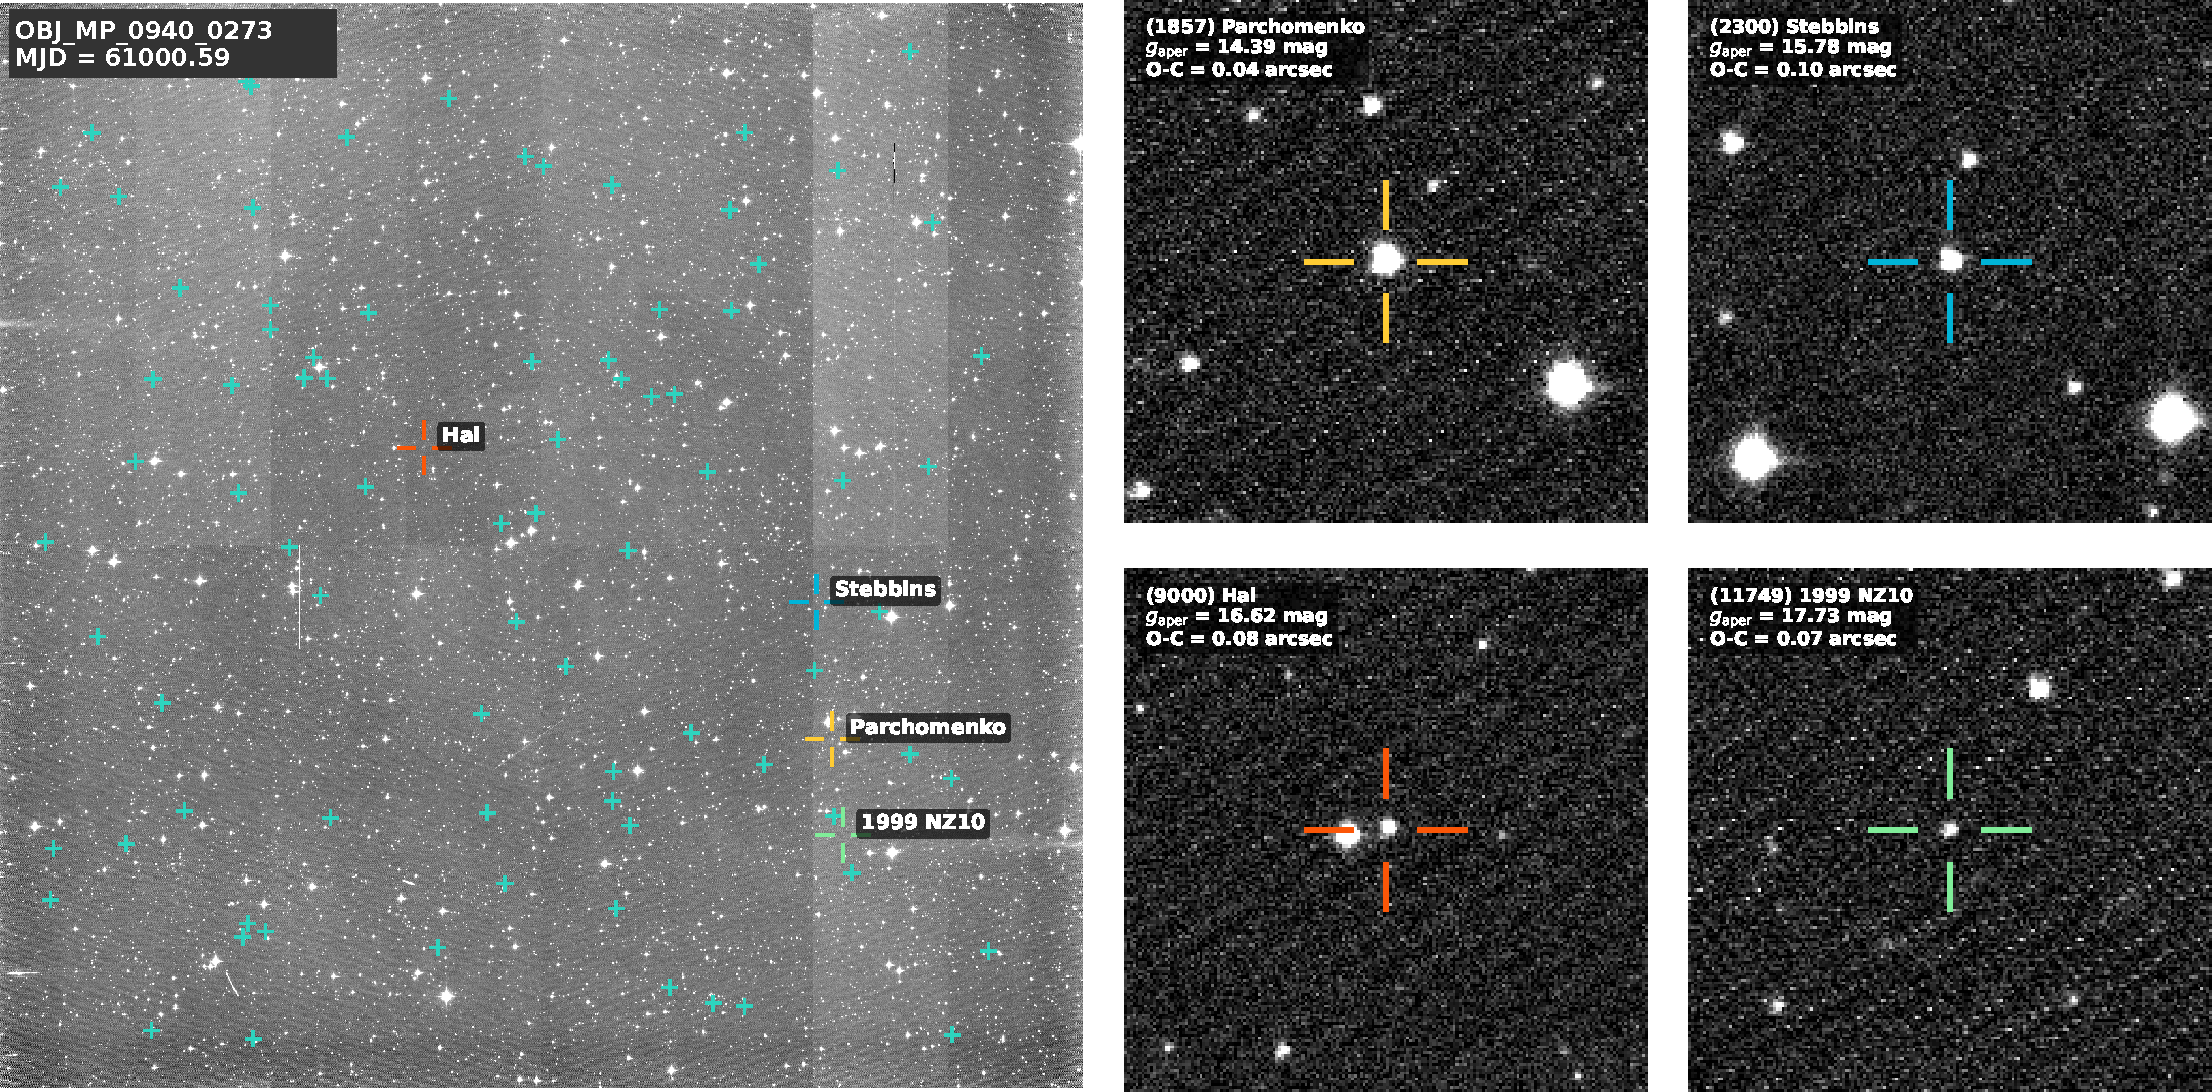
\includegraphics[width=0.98\linewidth]{fig01_exposure.pdf}
\caption{A 30~s white-light exposure obtained on 2025 November~21.
The wide-field panel marks four known-asteroid associations, and the
cutouts show their measured positions. Labels give the calibrated
white-light aperture magnitude \gaper\ and radial
observed-minus-computed (O$-$C) separation. The displayed MJD is
the exposure start, rounded for display; asteroid positions are
compared at the exposure midpoint using the full time precision.
The image uses a z-scale display with local background treatment.}
\label{fig:exposure}
\end{figure}

\begin{table}[tbp]
\centering
\caption{Instrument and Standard Survey Parameters}
\label{tab:design}
\begin{tabular}{ll}
\toprule
Quantity & Value or convention\\
\midrule
Telescope & Xinglong 60/90~cm Schmidt, $f/3$\\
Detector size & $9,216\times9,232$ pixels\\
Pixel size / readout channels & $10~\mu$m / 16\\
Typical pixel scale & $1.15\asec$~pixel$^{-1}$\\
Nominal field of view & $2.94^\circ\times2.95^\circ$\\
Observing band & $W$ (white light)\\
Reported magnitude & Calibrated aperture magnitude \gaper\\
Measurement aperture & Eight-pixel diameter\\
Field library & 1,855 ecliptic fields\\
Standard exposure & 30~s\\
Nominal visits / interval & Three visits / $\sim30$~min\\
Scheduled readout allowance & 15~s\\
Minimum planned target altitude & $30^\circ$\\
Prediction magnitude limit & $V<22.5$\\
Primary / auxiliary association radius & $1.0\asec$ / $1.5\asec$\\
Motion-search angular-rate range & $3$--$63$~\rateunit\\
\bottomrule
\end{tabular}
\end{table}

\subsection{Observing strategy and the first-year sample}
\label{sec:design}
\label{sec:cohorts}

The field library contains 1,855 pointings with ecliptic latitudes
between approximately $-18.5^\circ$ and $+16.3^\circ$. Each night's
plan selects fields using altitude, seasonal visibility, Moon
separation, and previous coverage. Nearby fields are grouped to
limit slews. A standard sequence aims for three visits to each field,
with a nominal interval of 30~min between repeat starts. The
scheduling allowance includes 15~s for readout in addition to the
30~s exposure and pointing overheads.

The first-year sample covers 2025 November~15 to 2026 November~15.
An observing night begins at local noon in Beijing time (UTC+8) and
ends at noon on the following day; it is labeled by its starting
date. We include night labels from 2025 November~15 through 2026
November~14. The last night therefore includes the morning of 2026
November~15. Exposure membership is determined from the midpoint
time. This definition treats each night's repeated observations as
a continuous sequence.

Other filters and observing modes occur in the archive, including the
2026 November 11--13 observations. They are tabulated separately and
are excluded from the homogeneous standard-survey measurements below.
We select distinct standard 30~s white-light exposures with calibrated
source measurements, reliable timing, and WCS solutions consistent
with the camera geometry. Images repeated in more than one directory
are counted once. The selection retains the range of image quality
and sky conditions encountered during the survey. It contains
\yrNexp\ exposures on \yrNnight\ observing nights. All first-year
coverage, cadence, photometric, and asteroid measurements below
refer to this exposure sample, with the additional source selections
specified for each measurement. Field sampling is determined from
the observed pointings and exposure times, including interrupted
and extended observing sequences.
